\documentclass[tikz, border=2pt]{standalone} % Use standalone class with tikz option
\usepackage{xcolor}
\usepackage{amsmath} % Needed for \mathcal if you use it, good practice anyway
% Make sure ALL needed libraries are loaded
\usetikzlibrary{positioning, arrows.meta, shapes.geometric, fit, backgrounds, calc} 

% Define custom colors
\definecolor{lightgreen}{RGB}{200, 230, 200}
\definecolor{lightblue}{RGB}{173, 216, 230} % Standard light blue
\definecolor{lighterblue}{RGB}{211, 225, 245} % Even lighter blue for projection
\definecolor{lightpink}{RGB}{245, 200, 195} % Salmon/coral color

% Define dimension for matrix cell size globally or before tikzpicture
\newdimen\celldim 

\begin{document}

% No \begin{figure}, \centering, \caption, or \label here

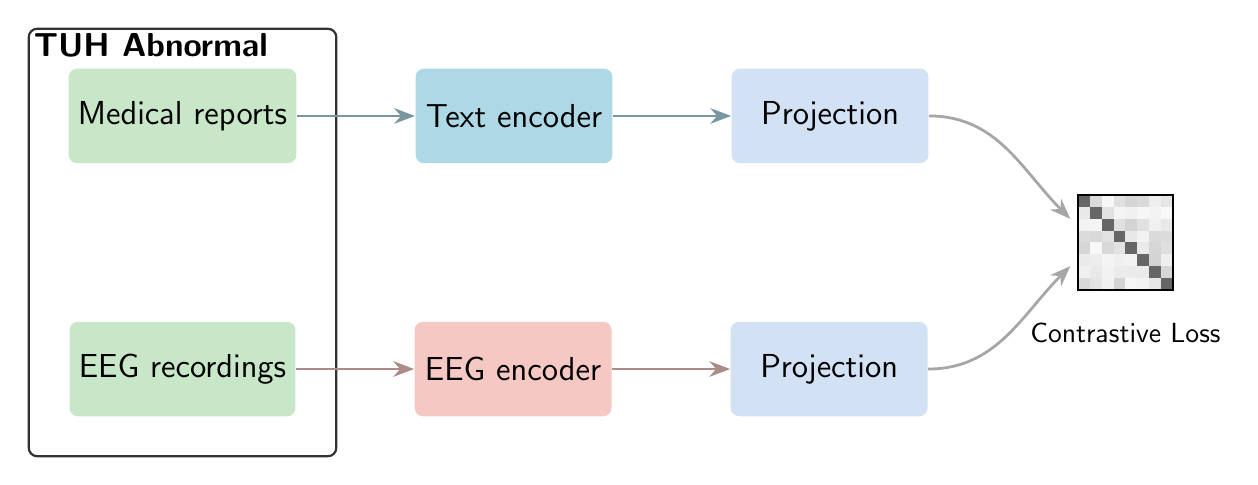
\begin{tikzpicture}[
    node distance=1cm and 1.5cm, % Vertical and horizontal node distance
    >=Stealth, % Arrow tip style
    box/.style={ % Style for main boxes, takes fill color as argument
        rectangle,
        rounded corners=3pt, % Slightly smaller rounding
        minimum width=2.5cm,
        minimum height=1.2cm, % Adjusted height slightly
        text centered,
        font=\sffamily\large,
        draw=none, % No border, fill provides shape
        fill=#1
    },
    % Specific styles using the base 'box' style
    input/.style={box=lightgreen},
    text_encoder/.style={box=lightblue, text=black}, % Specify text color if needed
    eeg_encoder/.style={box=lightpink, text=black},  % Specify text color if needed
    projection/.style={box=lighterblue}, % Simple rectangle projection
    % Arrow style
    arrow/.style={
        ->, 
        thick,
        line width=1pt,
        draw=#1 % Make arrow color an argument
    },
    % Default arrow color (if not specified later)
    arrow/.default=black,
    % Style for labels
    label_text/.style={ 
        font=\sffamily, 
        text centered, 
        align=center
    }
]

% Input blocks
\node[input] (medical) {Medical reports};
\node[input] (eeg) [below=2.0cm of medical] {EEG recordings}; % Adjusted spacing

% Encoder blocks
\node[text_encoder] (text_enc) [right=1.5cm of medical] {Text encoder};
\node[eeg_encoder] (eeg_enc) [right=1.5cm of eeg] {EEG encoder};

% Projection blocks (Using simple rectangle style 'projection')
\node[projection] (proj1) [right=1.5cm of text_enc] {Projection};
\node[projection] (proj2) [right=1.5cm of eeg_enc] {Projection};

% Draw arrows (Pass color to the arrow style)
% Using slightly darkened versions of the fill colors for arrows
\draw[arrow=lightblue!70!black] (medical) -- (text_enc); 
\draw[arrow=lightblue!70!black] (text_enc.east) -- (proj1.west); % Adjusted anchor name for clarity
\draw[arrow=lightpink!70!black] (eeg) -- (eeg_enc);
\draw[arrow=lightpink!70!black] (eeg_enc.east) -- (proj2.west); % Adjusted anchor name for clarity

% --- Start: Correlation Matrix for Contrastive Loss ---
% Calculate center position for the matrix where loss text was
\coordinate (matrix_center) at ($(proj1.east)!0.5!(proj2.east) + (2.5cm, 0)$); 
% Matrix parameters - Use size similar to projection height
\def\matrixsize{1.2cm} 
\def\N{8} % Number of cells per side (NxN matrix)
\pgfmathsetlength{\celldim}{\matrixsize/\N} % Calculate the cell dimension

% Draw the matrix using nested loops within a scope
\begin{scope}[shift={(matrix_center)}, xshift=-0.5*\matrixsize, yshift=0.5*\matrixsize] % Shift origin to top-left
    \foreach \i in {1,...,\N} { % Row index
        \foreach \j in {1,...,\N} { % Column index
            % Calculate numerical multipliers first
            \pgfmathtruncatemacro{\xmultiplier}{\j-1} 
            \pgfmathtruncatemacro{\ymultiplier}{-\i}  
            % Define the coordinate using the multipliers and the dimension
            \coordinate (cellpos) at (\xmultiplier*\celldim, \ymultiplier*\celldim);

            % Determine color string 
            \pgfmathparse{(\i == \j) ? 0 : 1} 
            \ifdim\pgfmathresult pt=0pt 
                \edef\cellfillcolor{black!60} % Slightly lighter diagonal 
            \else
                \pgfmathsetmacro{\randompercent}{rnd*30+5} % Lighter random grays
                \edef\cellfillcolor{gray!\randompercent} 
            \fi

            % Draw the filled cell
            \fill[\cellfillcolor] (cellpos) rectangle ++(\celldim, \celldim);
        }
    }
    % Draw border around the matrix
    \draw[thick] (0,0) rectangle (\matrixsize, -\matrixsize); 
\end{scope} % End of matrix scope

% Add Label below the matrix
\node[label_text, below=0.9cm of matrix_center] {Contrastive Loss}; % Adjusted spacing below matrix

% Use slightly curved arrows pointing towards the MATRIX edge
\draw[arrow=gray!70] (proj1.east) to [out=0, in=135] ($(matrix_center)+(-0.5*\matrixsize-0.1cm, 0.25*\matrixsize)$); 
\draw[arrow=gray!70] (proj2.east) to [out=0, in=225] ($(matrix_center)+(-0.5*\matrixsize-0.1cm, -0.25*\matrixsize)$);
% --- End: Correlation Matrix ---


% Outer container box using background layer and label
\begin{pgfonlayer}{background}
    \node[
        draw=black!80, % Slightly softer black border
        thick, 
        rectangle, 
        rounded corners=3pt, % Match node rounding
        inner sep=0.5cm, % Padding inside box
        fit=(medical) (eeg), % Fit around these nodes
        label={[font=\sffamily\large\bfseries, anchor=north west, inner sep=2pt]north west:TUH Abnormal} % Use label option
    ] (tuh) {}; 
\end{pgfonlayer}

\end{tikzpicture}

\end{document}